\documentclass[a4paper, 12pt]{article}

\usepackage{bera}% optional: just to have a nice mono-spaced font
\usepackage{listings}
\usepackage{xcolor}
\usepackage{tikz}

\usepackage{listings}
\usepackage{color}
\usepackage{booktabs, makecell, colortbl}

\definecolor{dkgreen}{rgb}{0,0.6,0}
\definecolor{gray}{rgb}{0.5,0.5,0.5}
\definecolor{mauve}{rgb}{0.58,0,0.82}
\definecolor{gray}{rgb}{0.4,0.4,0.4}
\definecolor{darkblue}{rgb}{0.0,0.0,0.6}
\definecolor{lightblue}{rgb}{0.0,0.0,0.9}
\definecolor{cyan}{rgb}{0.0,0.6,0.6}
\definecolor{darkred}{rgb}{0.6,0.0,0.0}


\colorlet{punct}{red!60!black}
\definecolor{background}{HTML}{EEEEEE}
\definecolor{delim}{RGB}{20,105,176}
\colorlet{numb}{magenta!60!black}

\lstdefinelanguage{json}{
    basicstyle=\normalfont\ttfamily,
    numbers=left,
    numberstyle=\scriptsize,
    stepnumber=1,
    numbersep=8pt,
    showstringspaces=false,
    breaklines=true,
    frame=lines,
    backgroundcolor=\color{background},
    literate=
     *{0}{{{\color{numb}0}}}{1}
      {1}{{{\color{numb}1}}}{1}
      {2}{{{\color{numb}2}}}{1}
      {3}{{{\color{numb}3}}}{1}
      {4}{{{\color{numb}4}}}{1}
      {5}{{{\color{numb}5}}}{1}
      {6}{{{\color{numb}6}}}{1}
      {7}{{{\color{numb}7}}}{1}
      {8}{{{\color{numb}8}}}{1}
      {9}{{{\color{numb}9}}}{1}
      {:}{{{\color{punct}{:}}}}{1}
      {,}{{{\color{punct}{,}}}}{1}
      {\{}{{{\color{delim}{\{}}}}{1}
      {\}}{{{\color{delim}{\}}}}}{1}
      {[}{{{\color{delim}{[}}}}{1}
      {]}{{{\color{delim}{]}}}}{1},
}

\lstset{
  basicstyle=\ttfamily\footnotesize,
  columns=fullflexible,
  showstringspaces=false,
  numbers=left,                   % where to put the line-numbers
  numberstyle=\tiny\color{gray},  % the style that is used for the line-numbers
  stepnumber=1,
  numbersep=5pt,                  % how far the line-numbers are from the code
  backgroundcolor=\color{white},      % choose the background color. You must add \usepackage{color}
  showspaces=false,               % show spaces adding particular underscores
  showstringspaces=false,         % underline spaces within strings
  showtabs=false,                 % show tabs within strings adding particular underscores
  frame=none,                   % adds a frame around the code
  rulecolor=\color{black},        % if not set, the frame-color may be changed on line-breaks within not-black text (e.g. commens (green here))
  tabsize=2,                      % sets default tabsize to 2 spaces
  captionpos=b,                   % sets the caption-position to bottom
  breaklines=true,                % sets automatic line breaking
  breakatwhitespace=false,        % sets if automatic breaks should only happen at whitespace
  title=\lstname,                   % show the filename of files included with \lstinputlisting;
                                  % also try caption instead of title  
  commentstyle=\color{gray}\upshape
}


\lstdefinelanguage{XML}
{
  morestring=[s][\color{mauve}]{"}{"},
  morestring=[s][\color{black}]{>}{<},
  morecomment=[s]{<?}{?>},
  morecomment=[s][\color{dkgreen}]{<!--}{-->},
  stringstyle=\color{black},
  identifierstyle=\color{lightblue},
  keywordstyle=\color{red},
  morekeywords={xmlns,xsi,noNamespaceSchemaLocation,type,id,x,y,source,target,version,tool,transRef,roleRef,objective,eventually}% list your attributes here
}

\usepackage[utf8]{inputenc}
\usepackage[T1]{fontenc}
\usepackage[french]{babel}
\usepackage{graphicx}
\usepackage{amsmath}
\usepackage{hyperref}
\usepackage{lmodern}
\usepackage{moreverb}
\usepackage{multicol}
% Please add the following required packages to your document preamble:
 \usepackage[table,xcdraw]{xcolor}
% If you use beamer only pass "xcolor=table" option, i.e. \documentclass[xcolor=table]{beamer}
 \usepackage[normalem]{ulem}
\useunder{\uline}{\ul}{}



\usepackage[a4paper,left=2cm,right=2cm,top=2cm,bottom=2cm]{geometry}

\pagestyle{headings}
\pagestyle{plain}


\setcounter{secnumdepth}{4}
\setcounter{tocdepth}{4}
\makeatletter


\makeatother



\makeatletter
\def\toclevel@subsubsubsection{4}
\def\toclevel@paragraph{5}
\def\toclevel@subparagraph{6}
\makeatother


\setlength{\parindent}{0cm}
\setlength{\parskip}{1ex plus 0.5ex minus 0.2ex}
\newcommand{\hsp}{\hspace{20pt}}
\newcommand{\HRule}{\rule{\linewidth}{0.5mm}}



\begin{document}

\begin{titlepage}
  \begin{sffamily}
  \begin{center}

   
  \textsc{\LARGE }\\[2cm]

    \textsc{\Large Suivi de projet}

    % Title
    \HRule \\[0.4cm]
    { \huge  \textsc{Projet d'interopérabilité} \\
    \textsc{\small Groupe 4}\\ [0.4cm] }
	

    \HRule \\[2cm]
    \textsc {Idriss BENGUEZZOU\\ Iness BOUABID\\Ali BOUGASSAA\\Ghilas MEZIANE }
 \begin{figure}
     \centering
    
\includegraphics[scale=0.2]{logoUJM.png}
     \label{fig:ujm_logo}
 \end{figure}
   
    \

    \vfill

    % Bottom of the page
    {\large {} 08/02/2023}

  \end{center}
  \end{sffamily}
\end{titlepage}


\newpage
\tableofcontents

\newpage
\section{Objet du document}

L'objectif de ce document de suivi de projet est de fournir une vue d'ensemble des progrès du projet, en mettant l'accent sur deux aspects clés : la révision des tâches et le planning du reste à faire.

La première partie de ce document se concentrera sur la révision des tâches. Elle fournira une liste détaillée de toutes les tâches du projet, avec une évaluation de l'état d'avancement de chaque tâche. 

La deuxième partie de ce document sera consacrée au planning du reste à faire. Elle fournira une liste des tâches restantes à accomplir, ainsi que des dates d'échéance pour chaque tâche. Cette liste sera mise à jour régulièrement pour refléter les changements dans le projet et les progrès réalisés. 

\section{Révision des tâches}

Voici la liste des tâches actuelles du projet, ainsi que leur état d'avancement :

\subsection{Interrogation de la Wikibase}

\begin{center}
    
\begin{tabular}{|p{14cm}|p{3cm}|}
\hline
\rowcolor[HTML]{EFEFEF}
Intitulé de la tâche & État d'avancement \\ 
\hline
Création d'un formulaire pour les requêtes utilisateur & Terminé \\
\hline
Mise en place de la fonctionnalité de recherche de base pour trouver des lieux culturels & Terminé \\
\hline
Configuration de docker-compose.yml pour pouvoir utiliser des requêtes SPARQL & Terminé \\
\hline
Création d'un script pour convertir les données récupérées des requêtes SPARQL en un format commun pour une utilisation facile par l'application & En cours \\
\hline
Validation des critères de recherche soumis pour s'assurer que les informations fournies sont correctes et complètes & En cours \\
\hline
Utilisation des requêtes SPARQL pour récupérer les résultats correspondant aux critères de recherche soumis par l'utilisateur & En cours \\
\hline
Mise en place de l'affichage des résultats de la recherche pour les utilisateurs & En cours \\
\hline
Mise en place de la navigation dans les résultats de recherche pour permettre aux utilisateurs de parcourir les résultats & En cours \\
\hline
Mise en place de la gestion des erreurs pour informer l'utilisateur si une requête échoue ou ne renvoie aucun résultat & En cours \\ \hline
\end{tabular}
\end{center}
\newpage


\subsection{Injection de données}


\subsubsection{Source de données}
\textbf{API}

\begin{tabular}{|p{14cm}|p{3cm}|}
\hline
\rowcolor[HTML]{EFEFEF}
Intitulé de la tâche & État d'avancement \\
\hline Recherche et sélection de l'API la mieux adaptée pour les données que nous souhaitons récupérer. & Terminé. \\
\hline Développement d'un script Python pour interroger l'API et récupérer les données. & Terminé. \\
\hline Traitement des données récupérées pour les préparer à l'injection dans la Wikibase. & En cours.\\
\hline Développement d'un système de mise à jour des données pour garantir que les données de la Wikibase sont à jour avec les données de l'API. & En cours\\
\hline
\end{tabular}
\\

\textbf{CSV}

\begin{tabular}{|p{14cm}|p{3cm}|}
\hline
\rowcolor[HTML]{EFEFEF}
Intitulé de la tâche & État d'avancement \\
\hline Développement d'un script Python pour lire les données à partir des fichiers CSV. & Terminé \\
\hline Traitement des données pour les préparer à l'injection dans la Wikibase. & Terminé \\
\hline
\end{tabular}
\\\\

\textbf{Web}

\begin{tabular}{|p{14cm}|p{3cm}|}
\hline
\rowcolor[HTML]{EFEFEF}
Intitulé de la tâche & État d'avancement \\
\hline Identification des pages du site web contenant les données pertinentes. & Terminé \\
\hline Développement d'un script Python pour parcourir le site web et extraire les données. & Terminé \\
\hline Traitement des données pour les préparer à l'injection dans la Wikibase. & Terminé \\

\hline
\end{tabular}

Cette liste sera mise à jour régulièrement pour refléter l'état d'avancement actuel du projet.

\newpage
\section{Planning du reste à faire}

Voici la liste des tâches restantes à accomplir, avec leurs dates d'échéance prévues :

\begin{tabular}{|p{14cm}|p{3cm}|}
\hline
\rowcolor[HTML]{EFEFEF}
Intitulé de la tâche & Échéance \\
\hline
Développement d'un système de mise à jour des données pour garantir que les données de la Wikibase sont à jour avec les données du site web. & Reste à faire. \\
\hline Développement d'un système de mise à jour des données pour garantir que les données de la Wikibase sont à jour avec les données du fichier CSV. & Reste à faire. \\
\hline Création d'un parseur pour convertir une source de données dans un format commun. & Reste à faire. \\
\hline Mise en place du style de la page d'accueil & Reste à faire. \\
\hline Mise en place d'un système permettant de mettre à jour les données dans la Wikibase depuis une source externe. & Reste à faire. \\ 
\hline Ajout de fonctionnalités pour gérer les conflits en cas de modifications simultanées des mêmes données par plusieurs utilisateurs. & Reste à faire. \\ 
\hline
Mise en place de recherche avancée à l'aide de requêtes SPARQL & Reste à faire. \\

\hline
\end{tabular}


\begin{figure}[h]
    \centering
    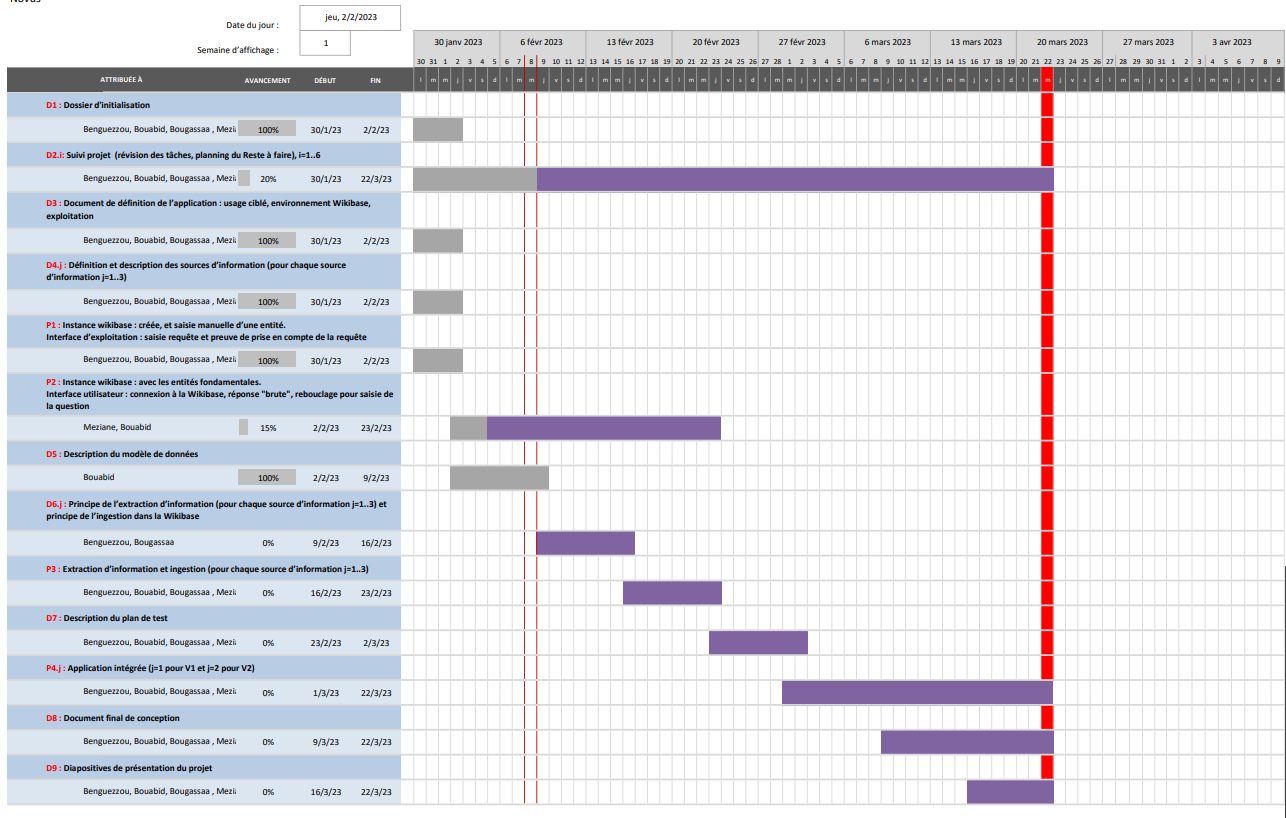
\includegraphics[scale=0.5]{diagramme.png}
    \caption{Gantt}
    \label{fig:my_label}
\end{figure}

\end{document}